
%%%%%%%%%%%%%%%%%%%%%%%%%%%%%%%%%%%%%%%%%%%%

\section{Définitions}
  \subsection{Observateur et référentiel}

Pour étudier un mouvement, un {\it observateur} doit mesurer la position de l'objet en mouvement au cours du temps. Il doit donc disposer d'une horloge (pour mesurer le temps) et d'un système de coordonnées spatiales (pour mesurer la position).

L'horloge et le système de coordonnées "attachés" à l'observateur est appelé {\it référentiel}


    \subsubsection{Exemple}
Un observateur détermine la vitesse du train en chronomètrant la durée mis par le train pour parcourir la distance séparant les deux arbres.

\begin{center}
%%%%%%%%%%%%%%%%%%%%%%%%%%%%%%%%%%%%%%%%%%%%%%%%%%%%%%%
%%%%%%%%%%%%%%%%%%%%%%%%%%%%%%%%%%%%%%%%%%%%%%%%%%%%%%%%%%%%%%%%%%%%
\def\scl{0.2}%scaling factor of the picture

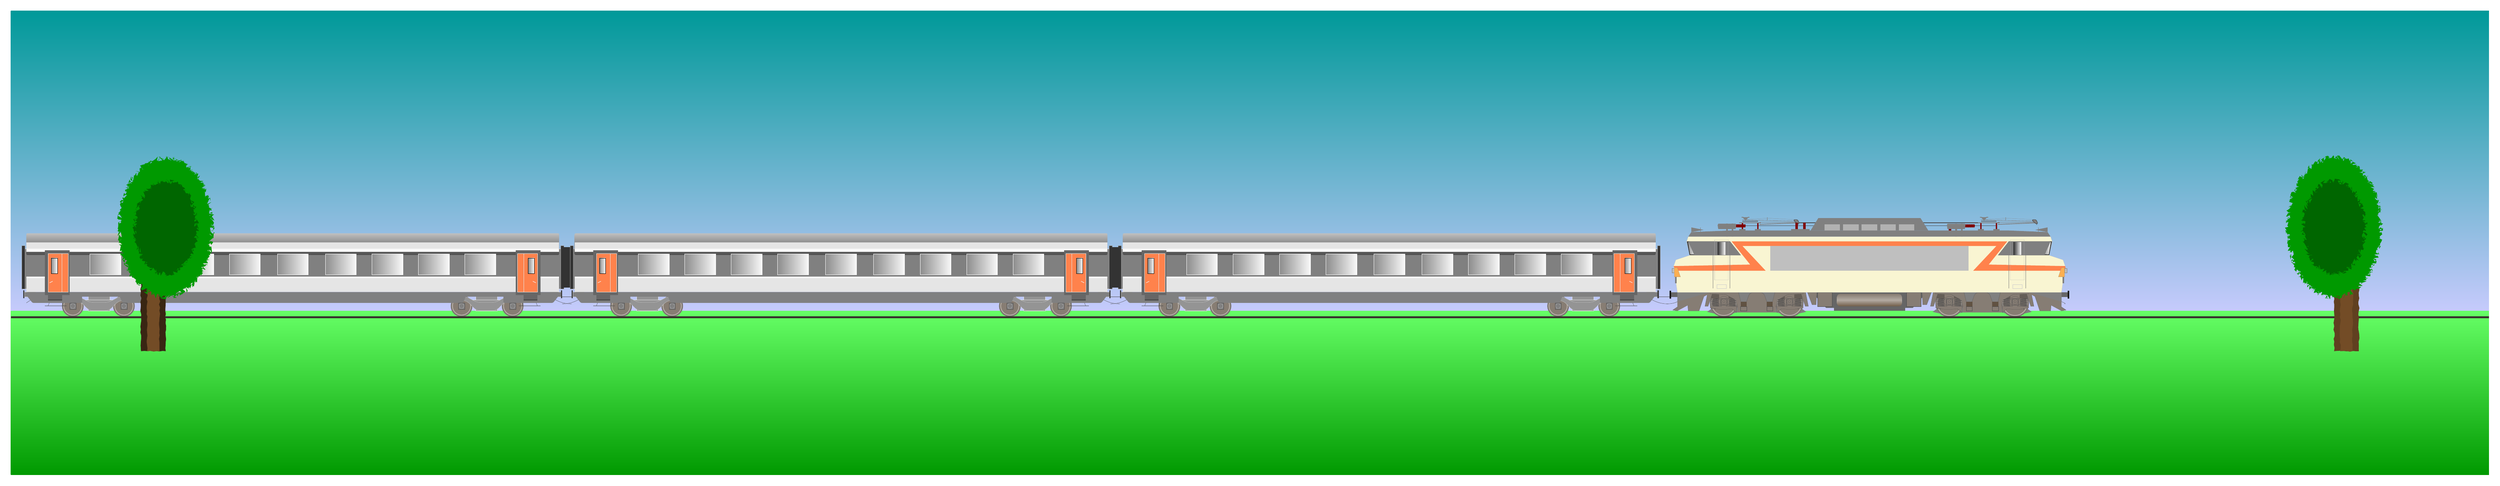
\begin{tikzpicture}[
  scale=\scl,
  beige/.style={color=gray!20!brown!40!yellow!20!},
  orange/.style={color=red!70!yellow!70!},
  wagon/.style={green!70!brown!20!black!75!,draw=black,thick},
  porte/.style={red!70!yellow!70!,draw=gray!20!, ultra thin},
  porteMotrice/.style={rounded corners = .1pt,draw=gray!60!, ultra thin},
  essieux/.style={gray!20!brown!30!black!60!,draw=black!70!, ultra thin},
  vitre/.style={bottom color=gray!5!, top color=gray!90!, shading angle={90}, draw=white, ultra thin},
  grisEssieux/.style={gray!20!brown!30!black!60!}
]


  \shade[bottom color=blue!20!white, top color=cyan!60!black] (20,10)
    rectangle (-60,0);
  \shade[bottom color=green!60!black, top color=green!60!] (20,-5)
    rectangle (-60,.3);



  \begin{scope}[xshift=0 cm,yshift=0 cm]%, scale = 0.3
%
%         LIAISONS
%
 \draw[black!70!, very thin] % liaison souple 42, rigide 65 +-11
    (6.1,0.65) to[out=330,in=0] (6.3,0.53);

 \draw[black!70!, very thin] 
    (-6.1,0.65) to[out=210,in=0] (-6.55,0.53);

 \draw[black!70!, thin] 
    (-6.1,0.76) -- (-6.56,0.76);


 % BUTOIRS
 %(\t * 6.1, 0.75) rectangle (\t * 6.4, 0.9);
 %(\t * 6.4, 0.7) rectangle (\t * 6.45, 0.95);

 % ESSIEUX derrière les roues

  \foreach \x in {3.64, -3.64}
   {
 \fill[gray] 
  (\x - 0.65, 0.95) -- (\x + 0.65, 0.95) --
 (\x + 1.6, 0.27) -- (\x + 1.06, 0.15) -- (\x + 0.65, 0.25)
 -- (\x - 0.65, 0.25) -- (\x - 1.06, 0.15) -- (\x - 1.6, 0.27) -- cycle;
  }

%  ROUES

\def\hauteur{0.55}% de l'axe des roues
\foreach \x in {2.58, 4.7, -4.7, -2.58}
  {
 % gris essieux : gray!20!brown!30!black!50!
    \fill[gray!20!brown!20!black!60!] (\x, \hauteur) circle (0.45 cm);
    \fill[gray!20!brown!40!black!40!] (\x, \hauteur) circle (0.41 cm);
    \fill[gray!10!brown!30!black!60!] (\x, \hauteur) circle (0.38 cm);

% RESSORT

  \foreach \t in {-1,1}
  {
     \draw[decorate, decoration={snake, segment length=1.5pt, amplitude=1.2mm}, black!70!, thin]
       (\x + \t * 0.28, 0.75) -- (\x + \t * 0.28, 0.35);
    % RESSORT fixation supérieur
     \fill[gray!20!brown!20!black!70!]
       (\x + \t * 0.28 - .13, 0.9) rectangle (\x + \t * 0.28 + .13, 0.7);
  }
  }


 % ESSIEUX devant les roues

\def\y{0.2}
  \foreach \x in {3.64, -3.64}
{
  \foreach \t in {-1,1}
  {
  % détail
 \fill[essieux] (\x + \t*1.57, 0.95) -- (\x + \t*1.67, 0.45) --
 (\x + \t*1.57, 0.45) -- (\x + \t*1.4, 0.95) -- cycle;

  %  montants supérieur
 \fill[essieux] (\x + \t*1.5, 0.95) -- (\x + \t*1.5, 0.85) -- (\x + \t*1, 0.83) -- (\x + \t*0.67, 0.65)
 -- (\x + \t*0.6, 0.35) -- (\x + \t*0.45, 0.35) -- (\x + \t*0.6, 0.95) -- cycle;


    %  montant inférieur
 \fill[essieux] (\x + \t * 1.5,0.45) -- (\x + \t * 1.5,0.4) -- (\x + \t * 1.2,0.35) -- (\x + \t * 1,0.35)
 -- (\x + \t * 0.80,0.37) -- (\x + \t * 0.65,0.25) -- (\x + \t * 0.65,0.45) -- cycle;

 \fill[essieux] (\x + \t*1.06, \hauteur + 0.05) circle (0.17 cm);
 \fill[grisEssieux]
 (\x + \t*1.06 + 0.16, 0.45) rectangle (\x + \t*1.06 + -0.16, 0.37);
 \fill[essieux]
 (\x + \t*1.06 + 0.1, \hauteur + 0.05 + -0.1) rectangle (\x + \t*1.06 + -0.1, \hauteur + 0.05 + 0.1);
    \fill[essieux] (\x + \t*1.06, \hauteur + 0.05) circle (0.09 cm);
    \fill[essieux] (\x + \t*1.06, \hauteur + 0.05) circle (0.04 cm);

  }

    %  milieux
   \fill[essieux, rounded corners = 3pt]
  (\x-0.22, 0.9) -- (\x + 0.22, 0.9) -- (\x + 0.4, 0.4) -- (\x - 0.4, 0.4) -- cycle;

    %  milieux inférieur 
  \fill[grisEssieux]
  (\x - 0.62,0.5) -- (\x + 0.62,0.5) -- (\x + 0.62,0.25) -- (\x - 0.62,0.25) -- cycle;

  \foreach \t in {-1,1}    % silent bloc
  {
  \fill[brown!30!black!80!]
 (\x + \t * 0.42 - 0.1, 0.6) rectangle (\x + \t * 0.42 + 0.1, 0.4);
  \fill[essieux]
 (\x + \t * 0.42 - 0.1, 0.45) rectangle (\x + \t * 0.42 + 0.1, 0.3);
  }
}

 % DESSOUS

 \fill[black!60!] 
  (1.9, 0.95) -- (- 1.9, 0.95) -- (- 1.4, 0.40) -- (1.4, 0.40) -- cycle;

  \shade[bottom color=gray!10!brown!50!black!60!, top color=gray!20!brown!40!black!40!] % ombre centre cylindre
  (1.05, 0.45) rectangle (-1.05, 0.66);
  \shade[bottom color=gray!20!brown!40!black!40!, top color=gray!10!brown!30!black!60!]
  (1.05, 0.64) rectangle (-1.05, 0.85);

 \fill[black!60!] 
  (2, 0.9) -- (- 2, 0.9) -- (- 1.9, 0.75) -- (1.9, 0.75) -- cycle;
 \fill[black!60!] 
  (1.15, 0.55) -- (- 1.15, 0.55) -- (- 1.15, 0.3) -- (1.15, 0.3) -- cycle;


  \shade[bottom color=brown!40!black!80!, top color=gray!20!brown!40!black!40!, rounded corners = 3pt]% cylindre
  (1.05, 0.45) rectangle (-1.05, 0.66);
  \shade[bottom color=gray!20!brown!40!black!40!, top color=gray!10!brown!30!black!60!, rounded corners = 3pt]%, shading angle={90}
  (1.05, 0.64) rectangle (-1.05, 0.85);

  \foreach \t in {-1,1}
{
  \fill[essieux] % details 1
 (\t * 2, 0.9) -- (\t * 1.7, 0.9) -- (\t * 1.72, 0.5)
 -- (\t * 1.85, 0.5) --  cycle;
  \fill[essieux] % details 2
 (\t * 1.67, 0.9) -- (\t * 1.2, 0.9) -- (\t * 1.2, 0.45)
 -- (\t * 1.67, 0.45) --  cycle;
}

 % BUTOIRS
\foreach \t in {-1,1}
{
  \fill[color=gray!80!black] % 
 (\t * 6.1, 0.75) rectangle (\t * 6.4, 0.9);
  \fill[color=black!80!gray] % plaques
 (\t * 6.4, 0.7) rectangle (\t * 6.45, 0.95);
}

% BAS DE CAISSE

\foreach \t in {-1,1}
{

  \fill[essieux] % details
 (\t * 5.9, 0.9) -- (\t * 5.3, 0.9) -- (\t * 5.5, 0.3)
 -- (\t * 5.85, 0.3) --  cycle;

  \fill[essieux] % pare bufle
 (\t * 6.2, 0.43) -- (\t * 6.35, 0.33) -- (\t * 6.2, 0.3) --  cycle;
  \fill[grisEssieux] % pare bufle
 (\t * 5, 0.95) -- (\t * 6.2, 0.95) -- (\t * 6.2, 0.3) --  cycle;

  \fill[color=gray] % carrosserie
 (\t * 5, 0.95) -- (\t * 6.2, 0.95) -- (\t * 6.2, 0.6) --  cycle;
}


%
%     CORPS DE LA MOTRICE
%
% liaisons électriques entre caténaires
     \draw[black!70!, thin] (-2.4, 3.15) -- (3.9, 3.15);

     \draw[black!70!, thin] (-4.5, 3.05) -- (4.1, 3.05);


%isolant 1
  \foreach \x in {-4.1, -3.6, 3.6, 4.1}
     \draw[decorate, decoration={snake, segment length=.2pt, amplitude=0.2mm}, red!50!black, thin]
       (\x, 2.9) -- (\x, 3.15);
  \foreach \x in {-4.1, -3.6, 3.6, 4.1}
     \fill[gray]
       (\x - 0.1, 2.9) rectangle (\x + 0.1, 2.95);

%caténaire
\def\h{0.05}
  \foreach \x in {-4.1, 3.6}
  {
     \draw[gray, line width=.7pt] (\x + 0.6, 3.1+\h) -- (\x - 0.1, 3.1+\h);
     \draw[black!60!, line width=1pt] (\x + 0.5, 3.15+\h) -- (\x, 3.15+\h);

     \draw[gray, line width=.7pt] (\x + 0.55, 3.05+\h) -- (\x + 1.8, 3.1+\h);
     \draw[gray, line width=.1pt] (\x + 0.55, 3.13+\h) -- (\x  + 1.8, 3.13+\h);

     \draw[gray, line width=.3pt] (\x, 3.2+\h) -- (\x  + 1.8, 3.15+\h);
     \draw[gray, line width=.1pt] (\x, 3.2+\h) -- (\x  + .8, 3.25+\h) -- (\x  + 1.7, 3.2+\h);
     \draw[gray, line width=.3pt] (\x  + .8, 3.18+\h) -- (\x  + .8, 3.28+\h);

  \fill[gray, draw=black!70!, thin, rounded corners = 1pt]% coude
 (\x + 1.8, 3.05+\h) -- (\x + 1.83, 3.1+\h) -- (\x + 1.78, 3.2+\h) -- (\x + 1.65, 3.2+\h)
 -- (\x + 1.68, 3.15+\h) -- cycle;

  }
  \foreach \x in {-4, 3.7}
  {
  \fill[gray, line width=2pt]% support et capteurs
 (\x-0.1, 3.28+\h) -- (\x+0.1, 3.28+\h) -- (\x, 3.17+\h)  -- cycle;
     \draw[gray, line width=.7pt] (\x-0.07, 3.28+\h) -- (\x-0.13, 3.28+\h);
     \draw[gray, line width=.7pt] (\x+0.07, 3.28+\h) -- (\x+0.13, 3.28+\h);
  }

% ÉLÉMENTS CATÉNAIRES

%isolant 2 à gauche
  \foreach \x in {-2.1, -2.35}
     \draw[decorate, decoration={snake, segment length=.2pt, amplitude=.4mm}, red!50!black, thin]
       (\x, 2.9) -- (\x, 3.15);
     \fill[gray] (-2.23 - 0.3, 2.9) rectangle (-2.23 + 0.3, 2.95);
     \fill[gray] (-2.23 - 0.3, 2.9) rectangle (-2.23 + 0.3, 2.95);
%isolant 2 à droite
     \draw[decorate, decoration={snake, segment length=.2pt, amplitude=.4mm}, red!50!black, thin]
       (2.6, 2.9) -- (2.6, 3.08);
   %  \fill[gray] (2.6 - 0.3, 2.9) rectangle (2.6 + 0.3, 2.95);
% boitier
  \foreach \x in {-4.6, 2.8}
{
     \draw[decorate, decoration={snake, segment length=.2pt, amplitude=0.1mm}, red!50!black, thin]
       (\x+0.25, 3.05) -- (\x+0.6, 3.05);

     \fill[gray] (\x - 0.28, 3.12) -- (\x + 0.28, 3.12)
     -- (\x + 0.3, 3.07)
     -- (\x + 0.28, 2.95) -- (\x - 0.28, 2.95) -- (\x - 0.3, 3.07) -- cycle;

     \draw[gray, ultra thick] (\x + 0.18, 3.12) -- (\x + 0.18, 2.5);
     \draw[gray, ultra thick] (\x, 3.12) -- (\x, 2.5);
}


% trompes
\foreach \t in {-1, 1}
  {
  \fill[gray]%
 (\t * 5.35,2.92) -- (\t * 5.75, 3) -- (\t * 5.75, 2.85)  -- cycle;
  \draw[gray, thin] (\t * 5.45, 3) -- (\t * 5.45, 2.85);
  }


% TOIT

  \fill[color=black!50!] % toit 1
 (1.9, 2.9) -- (-1.9, 2.9) -- (-1.65, 3.3) -- (1.65, 3.3) -- cycle;
\def\demi{0.25}
\foreach \x in{ -1.2, -0.6, 0, 0.6, 1.2 }
  \fill[black!30!] % grilles
 (\x - \demi, 3.1) rectangle (\x + \demi, 2.9);

  \fill[color=gray] % toit 2
 (4.5, 2.9) -- (5.75, 2.85) -- (5.85, 2.7) -- (-5.85, 2.7) -- 
 (-5.75, 2.85) -- (-4.5, 2.9) -- cycle;

  \fill[beige,draw=gray!50!, ultra thin] % carosserie
 (5.85, 2.7) -- (5.9, 2.55) -- (5.8, 2.1) -- (6.25, 1.95) -- (6.32, 1.75)
 -- (6.2, 0.9) --  (-6.2, 0.9) -- (-6.32, 1.75) -- (-6.25, 1.95)
 -- (-5.8, 2.1) -- (-5.9, 2.55) -- (-5.85, 2.7) -- cycle;

  \fill[orange] % décoration
 (4.45, 2.55) -- (3.85, 1.8) -- (6.32, 1.75) -- (6.35, 1.6) -- (3.35, 1.6) -- (4.1, 2.4) 
 -- (-4.1, 2.4) -- (-3.35, 1.6) -- (-6.27, 1.6) -- (-6.32, 1.75) -- (-3.85, 1.8) -- (-4.45, 2.55) -- cycle;


  \fill[color=gray!50!] % grille
 (3.2,1.6) -- (3.2, 2.4) -- (-3.2,2.4) -- (-3.2, 1.6) --  cycle;

  %  FEUX

\foreach \t in {-1,1}
{
  \fill[color=gray!50!,draw=gray, ultra thin]
 (\t * 6.3,1.67) rectangle (\t * 6.37, 1.53);
  \fill[color=brown!20!red!50!yellow!70!,draw=gray, ultra thin]
 (\t * 6.2,1.7) -- (\t * 6.3, 1.7) -- (\t * 6.3, 1.4) -- (\t * 6.1, 1.4) -- cycle;
  \fill[color=gray]
 (\t * 6.23,1.4) rectangle (\t * 6.28, 1.2);
}


\foreach \t in {-1,1}
{
      % PARE BRISE ET GRIS AUTOUR

  \fill[color=gray] % gris
 (\t*4.5, 2.55) -- (\t*5.9, 2.55) -- (\t*5.8, 2.1) -- (\t*4.15, 2.1) --  cycle;
  \shade[bottom color=gray!5!, top color=gray!90!, shading angle={90}, draw=black] % vitre
 (\t*5.8, 2.54) -- (\t*5.87, 2.54) -- (\t*5.8, 2.12) -- (\t*5.6, 2.12) --  cycle;

  \fill[color=gray] % gris
 (\t*4.5, 2.55) -- (\t*5.85, 2.55) -- (\t*5.65, 2.1) -- (\t*4.15, 2.1) --  cycle;

      % PORTES

    \draw[porteMotrice]
 (\t*4.55, 1.3) rectangle (\t*5, 2.6);

    \draw[draw=gray!40!,very thin] % marches
 (\t*4.62, 1.03) rectangle (\t*4.93, 1.15);

    \draw[color=gray] (\t*4.5, 1.03) -- (\t*4.5, 2.3); % rampes
    \draw[color=gray] (\t*5.05, 1.03) -- (\t*5.05, 2.3);

  \shade[bottom color=white, top color=black!80!, shading angle={90}]
   (\t*4.65, 2.12) rectangle (\t*4.9, 2.52); % vitres
}

  % RAIL

  % RAIL
  \fill[color=brown!20!gray!40!black]
 %(-8.75, 0.02) rectangle (8.75, -0.05); WAGON
 (20, 0.13) rectangle (-6.7, 0.06);

  \end{scope}
%
%
%%%%%%%%%%%%%%%%%%%%%%%%%%%%%%%%%%%%%%%%%%%%%%%%%%%%%%%%%%%%%%%%%%%%%

         %    WAGONS

%%%%%%%%%%%%%%%%%%%%%%%%%%%%%%%%%%%%%%%%%%%%%%%%%%%%%%%%%%%%%%%%%%%%

  \begin{scope}[xshift=-15.5 cm,yshift=0.11 cm]%, scale = 0.3
%
%         LIAISONS
% 
  \fill[color=gray,draw=gray!20!, ultra thin] % fixation souflets
 (8.65, 0.9) rectangle (-8.65, 2.2);

 \draw[black!70!, very thin] % liaison souple
    (8.3,0.65) to[out=330,in=180] (9,0.42);
 \draw[black!70!, very thin] 
    (-8.3,0.65) to[out=210,in=0] (-9,0.42);

  \foreach \t in {-1, 1}
  {
  \fill[color=black!80!,draw=gray!80!, ultra thin] % 
 (8.65 * \t, 0.9) rectangle (8.75 * \t, 2.3); % gris foncé, souflets

    \coordinate (A) at (8.3 * \t,0.65) ;
    \coordinate (B) at (9 * \t,0.65) ;
 \draw[black!70!, thin] 
    (A) -- (B);

  }

 % BUTOIRS
  \foreach \t in {-1, 1}
  {
  \fill[color=gray,draw=gray!50!, ultra thin] % 
 (8.3 * \t, 0.65) rectangle (\t * 8.66, 0.8);
  \fill[color=gray!50!black] % 
 (\t * 8.66, 0.6) rectangle (\t * 8.7, 0.85);
  }
%
%     CORPS DU WAGON
%
  \shade[bottom color=black!70!, top color=gray!50!, rounded corners=1pt]  % toit
 (-8.6, 2) rectangle (8.6, 2.7);

  \fill[color=gray!20!] % gris clair
 (-8.6, 2.1) rectangle (8.6, 2.4);
  \fill[color=gray!20!] % gris clair
 (-8.6, 0.8) rectangle (8.6, 1.25);

  \fill[color=gray!5!] % blanc
 (-8.6, 2.1) rectangle (8.6, 2.2);
  \fill[color=gray!5!] % blanc
 (-8.6, 1.25) rectangle (8.6, 1.3);

%  ROUES

\def\hauteur{0.35}% de l'axe des roues
\foreach \x in {5.45, 7.1, -5.45, -7.1}
  {
 % gris essieux : gray!20!brown!30!black!50!
    \fill[gray!20!brown!20!black!60!] (\x, \hauteur) circle (0.35 cm);
    \fill[gray!20!brown!40!black!40!] (\x, \hauteur) circle (0.31 cm);
    \fill[gray!10!brown!30!black!60!] (\x, \hauteur) circle (0.28 cm);
  \fill[color=gray,draw=black!70!, ultra thin] %,rotate=45
 (\x + 0.1, \hauteur + -0.1) rectangle (\x -0.1, \hauteur + 0.1);

  \fill[color=gray,draw=gray!20!, ultra thin] (\x, \hauteur) circle (0.08 cm);
  }
 % ESSIEUX
\def\y{0.2}
  \foreach \x in {6.25, -6.25}
   {
 \fill[black!20!gray!70!,draw=gray!20!, ultra thin] 
  (\x - 0.35, 0.2) rectangle (\x + 0.35, 0.45);

 \fill[black!20!gray!70!,draw=gray!20!, ultra thin] 
  (\x - 0.45, 0.45) rectangle (\x + 0.45, 0.55);

 \fill[black!20!gray!70!,draw=gray!20!, ultra thin] 
  (\x - 0.35, 0.55) rectangle (\x + 0.35, 0.7);

    \coordinate (A) at (\x + -0.75,\y + 0.45) ;
      \coordinate (B) at (\x - 0.2,\y + 0.27) ;
      \coordinate (C) at (\x + 0.2,\y + 0.27) ;
    \coordinate (D) at (\x + 0.75,\y + 0.45) ;
    \coordinate (E) at (\x + 0.75,\y + 0.32) ;
      \coordinate (F) at (\x + 0.2,\y + 0) ;
      \coordinate (G) at (\x - 0.2,\y + 0) ;
    \coordinate (H) at (\x - 0.75,\y + 0.32) ;
 \fill[black!20!gray!70!,draw=gray!20!, ultra thin] 
    (A) to[out=0,in=180] (B) to[out=0,in=180] (C) to[out=0,in=180]
    (D) to[out=-90,in=90] (E) to[out=180,in=0] (F) to[out=180,in=0]
    (G) to[out=180,in=0] (H) -- cycle;
  }

% MARCHE
  \foreach \t in {-1, 1}
  {
    \draw[draw=black!70!,very thin] % montant
 (\t * 7.9, 0.35) -- (\t * 7.8, 0.6);
    \draw[draw=black!70!,very thin] % montant
 (\t * 7.4, 0.35) -- (\t * 7.5, 0.6);
    \draw[draw=black!70!,thin] % marche
 (\t * 7.3, 0.35) -- (\t * 8, 0.35);
  }

% BAS DE CAISSE

  \fill[color=gray, rounded corners=1pt] % gris Foncé
    (-8.6, .8) rectangle (8.6, .65);


  \foreach \t in {-1, 1}
  \fill[color=gray, rounded corners=1pt] % gris Foncé
    (\t * 8.6, .7) -- (\t * 8.4, .45) -- (\t * 6.8, .45) -- (\t * 6.8, .7) -- cycle;
  \fill[color=gray, rounded corners=1pt] % gris Foncé
    (5.6, .7) -- (5.5, .45) -- (-5.5, .45) -- (-5.6, .7) -- cycle;

      % FENÊTRES
  \foreach \t in {1.05, 2.55, 4.05, 5.55}
  {
  \shade[vitre]
   (\t, 1.36) rectangle (\t + 1, 2.03);
  \shade[vitre]
   (-\t, 1.36) rectangle (-\t - 1, 2.03);
  }
  \shade[vitre]
   (-0.5, 1.36) rectangle (0.5, 2.03);

      % PORTES
  \foreach \t in {-1, 1}
  {

    \fill[gray!80!black] % marche
 (\t * 7.45, 0.53) rectangle (\t * 7.9, 0.7);
    \fill[gray!60!black] % marche
 (\t * 7.45, 0.53) rectangle (\t * 7.9, 0.57);

  \fill[gray!80!black]
 (\t * 7.2, 0.7) rectangle (\t * 8, 2.15);
  \fill[porte]
 (\t * 7.25, 0.8) rectangle (\t * 7.6, 2.05);
  \fill[porte]
 (\t * 7.45, 0.8) rectangle (\t * 7.9, 2.05);

  \shade[bottom color=gray!5!, top color=gray!90!, shading angle={90}, draw=black, ultra thin] % fenêtre
   (\t * 7.6, 1.4) rectangle (\t * 7.8, 1.9);

    \draw[gray!10!]
 (\t * 7.75, 1.15) -- (\t * 7.85, 1.1); % poignée
  }

  % RAIL WAGON
  \fill[color=brown!20!gray!40!black]
 (-8.85, 0.02) rectangle (8.85, -0.05);

  \end{scope}
%
%
%
%%%%%%%%%%%%%%%%%%%%%%%%%%%%%%%%%%%%%%%%%%%%%%%%%%%%%%%%%%%%%%%%%%%%%

         %    WAGON  2

%%%%%%%%%%%%%%%%%%%%%%%%%%%%%%%%%%%%%%%%%%%%%%%%%%%%%%%%%%%%%%%%%%%%

  \begin{scope}[xshift=-33.2 cm,yshift=0.11 cm]%, scale = 0.3
%
%         LIAISONS
% 
  \fill[color=gray,draw=gray!20!, ultra thin] % fixation souflets
 (8.65, 0.9) rectangle (-8.65, 2.2);

 \draw[black!70!, very thin] % liaison souple
    (8.3,0.65) to[out=330,in=180] (9,0.42);
 \draw[black!70!, very thin] 
    (-8.3,0.65) to[out=210,in=0] (-9,0.42);

  \foreach \t in {-1, 1}
  {
  \fill[color=black!80!,draw=gray!80!, ultra thin] % 
 (8.65 * \t, 0.9) rectangle (8.75 * \t, 2.3); % gris foncé, souflets
    \coordinate (A) at (8.3 * \t,0.65) ;
    \coordinate (B) at (9 * \t,0.65) ;
 \draw[black!70!, thin] 
    (A) -- (B);
  }

  \fill[color=black!80!] % 
 (8.75, 0.95) rectangle (8.95, 2.25); % gris foncé, souflet liaison
 % BUTOIRS
  \foreach \t in {-1, 1}
  {
  \fill[color=gray,draw=gray!50!, ultra thin] % 
 (8.3 * \t, 0.65) rectangle (\t * 8.66, 0.8);
  \fill[color=gray!50!black] % 
 (\t * 8.66, 0.6) rectangle (\t * 8.7, 0.85);
  }
%
%     CORPS DU WAGON
%
  \shade[bottom color=black!70!, top color=gray!50!, rounded corners=1pt]  % toit
 (-8.6, 2) rectangle (8.6, 2.7);

  \fill[color=gray!20!] % gris clair
 (-8.6, 2.1) rectangle (8.6, 2.4);
  \fill[color=gray!20!] % gris clair
 (-8.6, 0.8) rectangle (8.6, 1.25);

  \fill[color=gray!5!] % blanc
 (-8.6, 2.1) rectangle (8.6, 2.2);
  \fill[color=gray!5!] % blanc
 (-8.6, 1.25) rectangle (8.6, 1.3);

%  ROUES

\def\hauteur{0.35}% de l'axe des roues
\foreach \x in {5.45, 7.1, -5.45, -7.1}
  {
 % gris essieux : gray!20!brown!30!black!50!
    \fill[gray!20!brown!20!black!60!] (\x, \hauteur) circle (0.35 cm);
    \fill[gray!20!brown!40!black!40!] (\x, \hauteur) circle (0.31 cm);
    \fill[gray!10!brown!30!black!60!] (\x, \hauteur) circle (0.28 cm);
  \fill[color=gray,draw=black!70!, ultra thin] %,rotate=45
 (\x + 0.1, \hauteur + -0.1) rectangle (\x -0.1, \hauteur + 0.1);

  \fill[color=gray,draw=gray!20!, ultra thin] (\x, \hauteur) circle (0.08 cm);
  }
 % ESSIEUX
\def\y{0.2}
  \foreach \x in {6.25, -6.25}
   {
 \fill[black!20!gray!70!,draw=gray!20!, ultra thin] 
  (\x - 0.35, 0.2) rectangle (\x + 0.35, 0.45);

 \fill[black!20!gray!70!,draw=gray!20!, ultra thin] 
  (\x - 0.45, 0.45) rectangle (\x + 0.45, 0.55);

 \fill[black!20!gray!70!,draw=gray!20!, ultra thin] 
  (\x - 0.35, 0.55) rectangle (\x + 0.35, 0.7);

    \coordinate (A) at (\x + -0.75,\y + 0.45) ;
      \coordinate (B) at (\x - 0.2,\y + 0.27) ;
      \coordinate (C) at (\x + 0.2,\y + 0.27) ;
    \coordinate (D) at (\x + 0.75,\y + 0.45) ;
    \coordinate (E) at (\x + 0.75,\y + 0.32) ;
      \coordinate (F) at (\x + 0.2,\y + 0) ;
      \coordinate (G) at (\x - 0.2,\y + 0) ;
    \coordinate (H) at (\x - 0.75,\y + 0.32) ;
 \fill[black!20!gray!70!,draw=gray!20!, ultra thin] 
    (A) to[out=0,in=180] (B) to[out=0,in=180] (C) to[out=0,in=180]
    (D) to[out=-90,in=90] (E) to[out=180,in=0] (F) to[out=180,in=0]
    (G) to[out=180,in=0] (H) -- cycle;
  }

% MARCHE
  \foreach \t in {-1, 1}
  {
    \draw[draw=black!70!,very thin] % montant
 (\t * 7.9, 0.35) -- (\t * 7.8, 0.6);
    \draw[draw=black!70!,very thin] % montant
 (\t * 7.4, 0.35) -- (\t * 7.5, 0.6);
    \draw[draw=black!70!,thin] % marche
 (\t * 7.3, 0.35) -- (\t * 8, 0.35);
  }

% BAS DE CAISSE

  \fill[color=gray, rounded corners=1pt] % gris Foncé
    (-8.6, .8) rectangle (8.6, .65);


  \foreach \t in {-1, 1}
  \fill[color=gray, rounded corners=1pt] % gris Foncé
    (\t * 8.6, .7) -- (\t * 8.4, .45) -- (\t * 6.8, .45) -- (\t * 6.8, .7) -- cycle;
  \fill[color=gray, rounded corners=1pt] % gris Foncé
    (5.6, .7) -- (5.5, .45) -- (-5.5, .45) -- (-5.6, .7) -- cycle;

      % FENÊTRES
  \foreach \t in {1.05, 2.55, 4.05, 5.55}
  {
  \shade[vitre]
   (\t, 1.36) rectangle (\t + 1, 2.03);
  \shade[vitre]
   (-\t, 1.36) rectangle (-\t - 1, 2.03);
  }
  \shade[vitre]
   (-0.5, 1.36) rectangle (0.5, 2.03);

      % PORTES
  \foreach \t in {-1, 1}
  {

    \fill[gray!80!black] % marche
 (\t * 7.45, 0.53) rectangle (\t * 7.9, 0.7);
    \fill[gray!60!black] % marche
 (\t * 7.45, 0.53) rectangle (\t * 7.9, 0.57);

  \fill[gray!80!black]
 (\t * 7.2, 0.7) rectangle (\t * 8, 2.15);
  \fill[porte]
 (\t * 7.25, 0.8) rectangle (\t * 7.6, 2.05);
  \fill[porte]
 (\t * 7.45, 0.8) rectangle (\t * 7.9, 2.05);

  \shade[bottom color=gray!5!, top color=gray!90!, shading angle={90}, draw=black, ultra thin] % fenêtre
   (\t * 7.6, 1.4) rectangle (\t * 7.8, 1.9);

    \draw[gray!10!]
 (\t * 7.75, 1.15) -- (\t * 7.85, 1.1); % poignée
  }

  % RAIL WAGON
  \fill[color=brown!20!gray!40!black]
 (-8.85, 0.02) rectangle (8.85, -0.05);

  \end{scope}
%
%
%%%%%%%%%%%%%%%%%%%%%%%%%%%%%%%%%%%%%%%%%%%%%%%%%%%%%%%%%%%%%%%%%%%%%

         %    WAGON  3

%%%%%%%%%%%%%%%%%%%%%%%%%%%%%%%%%%%%%%%%%%%%%%%%%%%%%%%%%%%%%%%%%%%%

  \begin{scope}[xshift=-50.9 cm,yshift=0.11 cm]%, scale = 0.3
%
%         LIAISONS
% 
  \fill[color=gray,draw=gray!20!, ultra thin] % fixation souflets
 (8.65, 0.9) rectangle (-8.65, 2.2);

 \draw[black!70!, very thin] % liaison souple
    (8.3,0.65) to[out=330,in=180] (9,0.42);

 \draw[black!70!, very thin] 
    (-8.3,0.65) -- (-8.6,0.45);

  \foreach \t in {-1, 1}
  {
  \fill[color=black!80!,draw=gray!80!, ultra thin] % 
 (8.65 * \t, 0.9) rectangle (8.75 * \t, 2.3); % gris foncé, souflets
  }
  \fill[color=black!80!] % 
 (8.75, 0.95) rectangle (8.95, 2.25); % gris foncé, souflet liaison

    \coordinate (A) at (8.3,0.65) ;
    \coordinate (B) at (9,0.65) ;
 \draw[black!70!, thin] 
    (A) -- (B);

 % BUTOIRS
  \foreach \t in {-1, 1}
  {
  \fill[color=gray,draw=gray!50!, ultra thin] % 
 (8.3 * \t, 0.65) rectangle (\t * 8.66, 0.8);
  \fill[color=gray!50!black] % 
 (\t * 8.66, 0.6) rectangle (\t * 8.7, 0.85);
  }
%
%     CORPS DU WAGON
%
  \shade[bottom color=black!70!, top color=gray!50!, rounded corners=1pt]  % toit
 (-8.6, 2) rectangle (8.6, 2.7);

  \fill[color=gray!20!] % gris clair
 (-8.6, 2.1) rectangle (8.6, 2.4);
  \fill[color=gray!20!] % gris clair
 (-8.6, 0.8) rectangle (8.6, 1.25);

  \fill[color=gray!5!] % blanc
 (-8.6, 2.1) rectangle (8.6, 2.2);
  \fill[color=gray!5!] % blanc
 (-8.6, 1.25) rectangle (8.6, 1.3);

%  ROUES

\def\hauteur{0.35}% de l'axe des roues
\foreach \x in {5.45, 7.1, -5.45, -7.1}
  {
 % gris essieux : gray!20!brown!30!black!50!
    \fill[gray!20!brown!20!black!60!] (\x, \hauteur) circle (0.35 cm);
    \fill[gray!20!brown!40!black!40!] (\x, \hauteur) circle (0.31 cm);
    \fill[gray!10!brown!30!black!60!] (\x, \hauteur) circle (0.28 cm);
  \fill[color=gray,draw=black!70!, ultra thin] %,rotate=45
 (\x + 0.1, \hauteur + -0.1) rectangle (\x -0.1, \hauteur + 0.1);

  \fill[color=gray,draw=gray!20!, ultra thin] (\x, \hauteur) circle (0.08 cm);
  }
 % ESSIEUX
\def\y{0.2}
  \foreach \x in {6.25, -6.25}
   {
 \fill[black!20!gray!70!,draw=gray!20!, ultra thin] 
  (\x - 0.35, 0.2) rectangle (\x + 0.35, 0.45);

 \fill[black!20!gray!70!,draw=gray!20!, ultra thin] 
  (\x - 0.45, 0.45) rectangle (\x + 0.45, 0.55);

 \fill[black!20!gray!70!,draw=gray!20!, ultra thin] 
  (\x - 0.35, 0.55) rectangle (\x + 0.35, 0.7);

    \coordinate (A) at (\x + -0.75,\y + 0.45) ;
      \coordinate (B) at (\x - 0.2,\y + 0.27) ;
      \coordinate (C) at (\x + 0.2,\y + 0.27) ;
    \coordinate (D) at (\x + 0.75,\y + 0.45) ;
    \coordinate (E) at (\x + 0.75,\y + 0.32) ;
      \coordinate (F) at (\x + 0.2,\y + 0) ;
      \coordinate (G) at (\x - 0.2,\y + 0) ;
    \coordinate (H) at (\x - 0.75,\y + 0.32) ;
 \fill[black!20!gray!70!,draw=gray!20!, ultra thin] 
    (A) to[out=0,in=180] (B) to[out=0,in=180] (C) to[out=0,in=180]
    (D) to[out=-90,in=90] (E) to[out=180,in=0] (F) to[out=180,in=0]
    (G) to[out=180,in=0] (H) -- cycle;
  }

% MARCHE
  \foreach \t in {-1, 1}
  {
    \draw[draw=black!70!,very thin] % montant
 (\t * 7.9, 0.35) -- (\t * 7.8, 0.6);
    \draw[draw=black!70!,very thin] % montant
 (\t * 7.4, 0.35) -- (\t * 7.5, 0.6);
    \draw[draw=black!70!,thin] % marche
 (\t * 7.3, 0.35) -- (\t * 8, 0.35);
  }

% BAS DE CAISSE

  \fill[color=gray, rounded corners=1pt] % gris Foncé
    (-8.6, .8) rectangle (8.6, .65);


  \foreach \t in {-1, 1}
  \fill[color=gray, rounded corners=1pt] % gris Foncé
    (\t * 8.6, .7) -- (\t * 8.4, .45) -- (\t * 6.8, .45) -- (\t * 6.8, .7) -- cycle;
  \fill[color=gray, rounded corners=1pt] % gris Foncé
    (5.6, .7) -- (5.5, .45) -- (-5.5, .45) -- (-5.6, .7) -- cycle;

      % FENÊTRES
  \foreach \t in {1.05, 2.55, 4.05, 5.55}
  {
  \shade[vitre]
   (\t, 1.36) rectangle (\t + 1, 2.03);
  \shade[vitre]
   (-\t, 1.36) rectangle (-\t - 1, 2.03);
  }
  \shade[vitre]
   (-0.5, 1.36) rectangle (0.5, 2.03);

      % PORTES
  \foreach \t in {-1, 1}
  {

    \fill[gray!80!black] % marche
 (\t * 7.45, 0.53) rectangle (\t * 7.9, 0.7);
    \fill[gray!60!black] % marche
 (\t * 7.45, 0.53) rectangle (\t * 7.9, 0.57);

  \fill[gray!80!black]
 (\t * 7.2, 0.7) rectangle (\t * 8, 2.15);
  \fill[porte]
 (\t * 7.25, 0.8) rectangle (\t * 7.6, 2.05);
  \fill[porte]
 (\t * 7.45, 0.8) rectangle (\t * 7.9, 2.05);

  \shade[bottom color=gray!5!, top color=gray!90!, shading angle={90}, draw=black, ultra thin] % fenêtre
   (\t * 7.6, 1.4) rectangle (\t * 7.8, 1.9);

    \draw[gray!10!]
 (\t * 7.75, 1.15) -- (\t * 7.85, 1.1); % poignée
  }

  % RAIL WAGON
  \fill[color=brown!20!gray!40!black]
 (-9.1, 0.02) rectangle (8.85, -0.05);

  \end{scope}
%
\tikzset{
  treetop/.style = {decoration={random steps, segment length=0.2mm}, decorate},
  trunk/.style   = {decoration={random steps, segment length=1mm,
                    amplitude=0.2mm}, decorate}}

%  arbre à droite
       \fill [brown!50!black, trunk] (15,-1) rectangle (15.8,2);
       \fill [brown!60!black, trunk] (15.2,-1) rectangle (15.6,2);
     
       \fill [green!60!black, treetop](15,3) ellipse (1.5 and 2.25);
       \fill [green!40!black, treetop](15,3) ellipse (1 and 1.5);
     

%  arbre à gauche
       \fill [brown!30!black, trunk] (-55,-1) rectangle (-55.8,3);
       \fill [brown!60!black, trunk] (-55.2,-1) rectangle (-55.6,3);
     
       \fill [green!60!black, treetop](-55,3) ellipse (1.5 and 2.25);
       \fill [green!40!black, treetop](-55,3) ellipse (1 and 1.5);
     

%
\end{tikzpicture}
%

%%%%%%%%%%%%%%%%%%%%%%%%%%%%%%%%%%%%%%%%%%%%%%%%%%%%%%
%%%%%%%%%%%%%%%%%%%%%%%%%%%%%%%%%%%%%%%%%%%%%%%%%%%%%%%%%%%%%%%%%%%%
\def\scl{1}%scaling factor of the picture


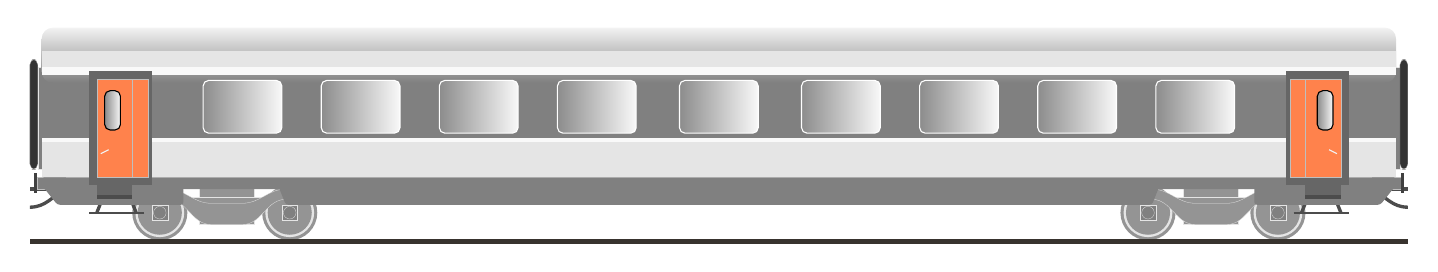
\begin{tikzpicture}[
  scale=\scl,
  %wagon/.style={yellow!30!brown!20!,rounded corners,draw=black,thick},
  wagon/.style={green!70!brown!20!black!75!,draw=black,thick},
 % toit/.style={black!70!brown!20!,draw=gray,thick},
  %roue/.style={brown!20!black!70!,draw=black,thick},
  fenetre/.style={white,rounded corners = 2pt,draw=black, thick},
  porte/.style={color=red!70!yellow!70!,draw=gray!50!, ultra thin}
  ]

  \begin{scope}[xshift=0 cm,yshift=0 cm]%, scale = 0.3
%
%         LIAISONS
% 
  \fill[color=gray,draw=gray!20!, ultra thin] % souflet gris
 (8.65, 0.9) rectangle (-8.65, 2.2);

 \draw[black!70!, very thick] 
    (8.3,0.65) to[out=330,in=180] (8.75,0.42);
 \draw[black!70!, very thick] 
    (-8.3,0.65) to[out=210,in=0] (-8.75,0.42);

  \foreach \t in {-1, 1}
  {
  \fill[color=black!80!,draw=gray!80!, ultra thin, rounded corners=2pt] % 
 (8.65 * \t, 0.9) rectangle (8.75 * \t, 2.3); % gris foncé, souflet

    \coordinate (A) at (8.3 * \t,0.65) ;
    \coordinate (B) at (8.75 * \t,0.65) ;
 \draw[black!70!, ultra thick] 
    (A) -- (B);

  }

 % BUTOIRS
  \foreach \t in {-1, 1}
  {
  \fill[color=gray,draw=gray!50!, ultra thin] % 
 (8.3 * \t, 0.65) rectangle (\t * 8.66, 0.8);
  \fill[color=gray!50!black] % 
 (\t * 8.66, 0.6) rectangle (\t * 8.7, 0.85);
  }
%
%     CORPS DU WAGON
%
  \shade[bottom color=gray, top color=gray!10!, rounded corners]  % toit
 (-8.6, 2) rectangle (8.6, 2.7);

  \fill[color=gray!20!] % gris clair
 (-8.6, 2.1) rectangle (8.6, 2.4);
  \fill[color=gray!20!] % gris clair
 (-8.6, 0.8) rectangle (8.6, 1.25);

  \fill[color=gray!5!] % blanc
 (-8.6, 2.1) rectangle (8.6, 2.2);
  \fill[color=gray!5!] % blanc
 (-8.6, 1.25) rectangle (8.6, 1.3);


% Arriere roues
  %\foreach \x in {6.25, -6.25} \fill[brown!40!black] (\x - 0.85, 0.8) rectangle (\x + 0.85, 0.45);

%  ROUES
\def\hauteur{0.35}% de l'axe des roues
\tikzset{
  roue/.pic={
    \fill[black!20!gray!70!] (0, \hauteur) circle (0.35 cm);
    \fill[gray!20!] (0, \hauteur) circle (0.31 cm);
    \fill[black!20!gray!70!] (0, \hauteur) circle (0.28 cm);

  \fill[color=gray,draw=gray!20!, ultra thin] %,rotate=45
 (0.1, \hauteur + -0.1) rectangle (-0.1, \hauteur + 0.1);

  \fill[color=gray,draw=gray!20!, ultra thin] (0, \hauteur) circle (0.08 cm);

  }
}

  \pic at (5.45,0)    {roue};
  \pic at (7.1,0)    {roue};
  \pic at (-5.45,0)    {roue};
  \pic at (-7.1,0)    {roue};
 % ESSIEUX
\def\y{0.2}
  \foreach \x in {6.25, -6.25}
   {
 \fill[black!20!gray!70!,draw=gray!20!, ultra thin] 
  (\x - 0.35, 0.2) rectangle (\x + 0.35, 0.45);

 \fill[black!20!gray!70!,draw=gray!20!, ultra thin] 
  (\x - 0.45, 0.45) rectangle (\x + 0.45, 0.55);

 \fill[black!20!gray!70!,draw=gray!20!, ultra thin] 
  (\x - 0.35, 0.55) rectangle (\x + 0.35, 0.7);

    \coordinate (A) at (\x + -0.75,\y + 0.45) ;
      \coordinate (B) at (\x - 0.2,\y + 0.27) ;
      \coordinate (C) at (\x + 0.2,\y + 0.27) ;
    \coordinate (D) at (\x + 0.75,\y + 0.45) ;
    \coordinate (E) at (\x + 0.75,\y + 0.32) ;
      \coordinate (F) at (\x + 0.2,\y + 0) ;
      \coordinate (G) at (\x - 0.2,\y + 0) ;
    \coordinate (H) at (\x - 0.75,\y + 0.32) ;
 \fill[black!20!gray!70!,draw=gray!20!, ultra thin] 
    (A) to[out=0,in=180] (B) to[out=0,in=180] (C) to[out=0,in=180]
    (D) to[out=-90,in=90] (E) to[out=180,in=0] (F) to[out=180,in=0]
    (G) to[out=180,in=0] (H) -- cycle;
  }

% MARCHE
  \foreach \t in {-1, 1}
  {
    \draw[draw=black!70!,very thick] % montant
 (\t * 7.9, 0.35) -- (\t * 7.8, 0.6);
    \draw[draw=black!70!,very thick] % montant
 (\t * 7.4, 0.35) -- (\t * 7.5, 0.6);
    \draw[draw=black!70!,thick] % marche
 (\t * 7.3, 0.35) -- (\t * 8, 0.35);
  }

% BAS DE CAISSE

  \fill[color=gray, rounded corners=1pt] % gris Foncé
    (-8.6, .8) rectangle (8.6, .65);


  \foreach \t in {-1, 1}
  \fill[color=gray, rounded corners=1pt] % gris Foncé
    (\t * 8.6, .7) -- (\t * 8.4, .45) -- (\t * 6.8, .45) -- (\t * 6.8, .7) -- cycle;
  \fill[color=gray, rounded corners=1pt] % gris Foncé
    (5.6, .7) -- (5.5, .45) -- (-5.5, .45) -- (-5.6, .7) -- cycle;

      % FENÊTRES
  \foreach \t in {1.05, 2.55, 4.05, 5.55}
  {
  \shade[bottom color=gray!5!, top color=gray!90!, shading angle={90},rounded corners=2pt, draw=white]
   (\t, 1.36) rectangle (\t + 1, 2.03);
  \shade[bottom color=gray!5!, top color=gray!90!, shading angle={90},rounded corners=2pt, draw=white]
   (-\t, 1.36) rectangle (-\t - 1, 2.03);
  }
  \shade[bottom color=gray!5!, top color=gray!90!, shading angle={90},rounded corners=2pt, draw=white]
   (-0.5, 1.36) rectangle (0.5, 2.03);

      % PORTES
  \foreach \t in {-1, 1}
  {

    \fill[gray!80!black] % marche
 (\t * 7.45, 0.53) rectangle (\t * 7.9, 0.7);
    \fill[gray!60!black] % marche
 (\t * 7.45, 0.53) rectangle (\t * 7.9, 0.57);

  \fill[gray!80!black]
 (\t * 7.2, 0.7) rectangle (\t * 8, 2.15);
  \fill[porte]
 (\t * 7.25, 0.8) rectangle (\t * 7.6, 2.05);
  \fill[porte]
 (\t * 7.45, 0.8) rectangle (\t * 7.9, 2.05);

  \shade[bottom color=gray!5!, top color=gray!90!, shading angle={90},rounded corners=2pt, draw=black] % fenêtre
   (\t * 7.6, 1.4) rectangle (\t * 7.8, 1.9);

    \draw[gray!10!]
 (\t * 7.75, 1.15) -- (\t * 7.85, 1.1); % poignée
  }

  % RAIL
  \fill[color=brown!20!gray!40!black]
 (-8.75, 0.02) rectangle (8.75, -0.05);

  \end{scope}
%
%
\end{tikzpicture}
%

\end{center}

L'observateur est immobile par rapport à la Terre, le mouvement est étudié dans le {\it référentiel terrestre}.

Un voyageur est assis dans le train, il observe le paysage défiler. Il se trouve dans le {\it référentiel lié au train} et peut également chronométrer la durée pour parcourir la distance entre les deux arbres, et ainsi déterminer la "vitesse du paysage" dans son régérentiel.


  \subsection{Mouvement rectiligne uniforme}

Un mouvement {\it rectiligne} est un mouvement en ligne droite. Un mouvement {\it uniforme} est un mouvement dont la vitesse est constante.

%%%%%%%%%%%%%%%%%%%%%%%%%%%%%%%%%%%%%%%%%%%{\it }



